% !TeX root = ../../../../01_git-vorgehensmodelle.tex

\subsection{Gitflow}
\label{sec:workflows:gitflow}

Ein weiteres Vorgehensmodell, welches versucht, die in \autoref{sec:einleitung} angesprochenen Probleme zu lösen, besteht in \emph{Gitflow}, welches \citeyear{driessenSuccessfulGitBranching2010} von Vincent Driessen entwickelt wurde~\cite{driessenSuccessfulGitBranching2010}.

Das Vorgehensmodell basiert auf einem zentralen \emph{Single\hyp Source\hyp of\hyp Truth} Repository, auf dem die langlebigen Branches liegen und meist \texttt{origin} genannt wird. Daher herrscht eine Push\hyp Pull\hyp Beziehung zwischen Entwickelnden und \texttt{origin}, wobei ein Austausch unter den Teams nicht ausgeschlossen ist~\cite{driessenSuccessfulGitBranching2010}.

Gitflow setzt auf dem Feature\hyp Branch\hyp Vorgehensmodell (vgl. \autoref{sec:workflows:branching}) auf. Es werden ebenfalls \texttt{main} als Haupt\hyp Branch und verschiedene Feature\hyp Branches verwendet. Zusätzlich wird ein zweiter langlebiger Branch -- \texttt{develop} -- und drei weitere unterstützende, kurzlebige Branch\hyp Arten -- Feature, Release und Hotfix -- definiert~\cite{driessenSuccessfulGitBranching2010}.

Den unterschiedlichen unterstützenden Branches wird je eine dedizierte Rolle zugeteilt. Diese unterliegen strikten Regeln zu deren Ursprung und Merge\hyp Ziel. Nach deren Merge in das jeweilige definierte Ziel werden die Branches wieder gelöscht~\cite{driessenSuccessfulGitBranching2010}.


\subsubsection{Langlebige Hauptbranches}

Die zwei Haupt\hyp Branches, welche eine unbeschränkte Lebensdauer haben, sind nach dem Gitflow\hyp Modell \texttt{master} (im Folgenden \texttt{main}~\cite{githubincRenamingDefaultBranch2022,softwarefreedomconservancyRegardingGitBranch2020}) und \texttt{develop}. Die Differenzierung begründet sich in den unterschiedlichen Rollen beider Branches.

Der \texttt{main}-Branch soll stets einen produktionsreifen Zustand darstellen und dient als Ausgangspunkt für den nächsten Release. Jeder Push auf \texttt{main} stellt per Definition einen \emph{Production-Release} dar, wodurch bspw. der Build und Roll-Out automatisierbar sind. Daher soll für jeden Merge auf \texttt{main} ein Tag mit einer Versionsnummer erstellt werden~\cite{driessenSuccessfulGitBranching2010}. Dadurch entspricht \texttt{main} der offiziellen Release\hyp Historie~\cite{atlassianGitflowWorkflow}.

Der \texttt{develop}-Branch stellt einen Integrationsbranch von Features dar, welcher die komplette Versionshistorie enthält~\cite{atlassianGitflowWorkflow}. Dabei sind alle einzelnen Features sichtbar, welche auf \texttt{main} zusammengefasst als ein Commit pro Release dargestellt werden.

Die jeweiligen Branches können entweder manuell (\texttt{git checkout -b \{develop, main\}}) oder mittels Git\hyp Erweiterung \texttt{git-flow}~\cite{driessenGitflow2012} erzeugt werden. Letzteres wird in \autoref{code:gitflow-init} dargestellt. Dabei werden alle relevanten Branches automatisch erstellt. Weitere Informationen zur Extension können unter \cite{kummerGitflowcheatsheet2023} eingesehen werden.

\begin{listing}
\inputminted[breaklines]{text}{src/assets/code/gitflow/gitflow_init.sh}
\caption{Initialisierung von Gitflow mittels \texttt{git-flow}-Extension}
\label{code:gitflow-init}
\end{listing}


\subsubsection{Feature-Branches}

Feature\hyp Branches werden von \texttt{develop} abgezweigt. Diese dienen dem gleichen Zweck, wie im Feature\hyp Branching\hyp Workflow: der Entwicklung von neuen Funktionen (vgl. \autoref{sec:workflows:branching}). Der zugehörige Release muss bei Beginn des Branches nicht zwingend bekannt sein~\cite{driessenSuccessfulGitBranching2010}, da der \texttt{develop}\hyp Branch dem Zwischenstand des \emph{nächsten} Releases entspricht~\cite{atlassianGitflowWorkflow}.

Der jeweilige Feature\hyp Branch kann entweder manuell mittels \texttt{git checkout -b <branch-name> develop} oder mittels \texttt{git flow feature start <branch-name>} erstellt werden~\cite{driessenGitflow2012}.

Nach Fertigstellung des dazugehörigen Features wird der Branch mittels no\hyp fast\hyp forward\hyp Merge (\verb|--no-ff|) oder \texttt{git flow feature finish <branch-name>} in \texttt{develop} integriert~\cite{driessenSuccessfulGitBranching2010,driessenGitflow2012}. Somit wird genau ein Commit\hyp Objekt pro Feature erstellt, wodurch nachvollziehbar ist, welcher Commit zu welchem Feature und vice versa gehört~\cite{driessenSuccessfulGitBranching2010}. Dadurch wird die Übersichtlichkeit erhöht und potenzielle Reverts vereinfacht. Allerdings sind die Commits dadurch größer, wodurch verschiedene Nachteile entstehen können, wie bspw. eine erhöhte Kompliziertheit beim Revert von fehlerhaften Commits.

Insgesamt verhält sich diese Branch\hyp Art identisch zum Feature\hyp Branching\hyp Modell (vgl. \autoref{sec:workflows:branching}) mit der Ausnahme, dass es es in Gitflow keinerlei Interaktion zu \texttt{main} gibt. Die Rolle von \texttt{main} im Feature\hyp Branching wird durch \texttt{develop} eingenommen.

Ein Beispiel für zwei Feature\hyp Branches ist in \autoref{fig:gitflow:feature} dargestellt. Dabei sind bereits zwei Features auf \texttt{develop} integriert, welche durch die beiden Commits angedeutet werden. Anschließend werden zwei Feature\hyp Branches von \texttt{develop} abgezweigt, auf denen parallel gearbeitet wird. Anschließend werden beide zurück in \texttt{develop} integriert.

\begin{figure}
    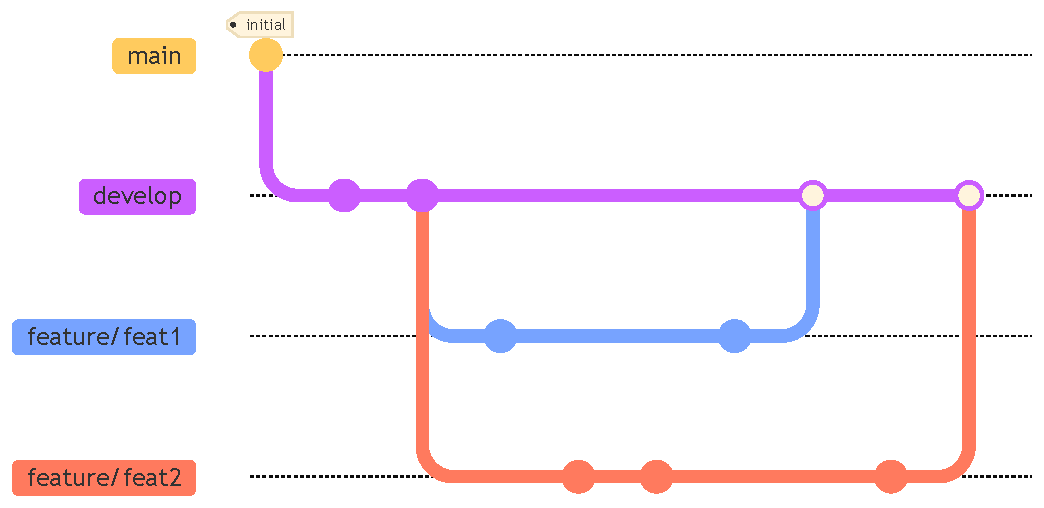
\includegraphics[width=0.45\textwidth]{src/assets/diagrams/gitflow/feature.pdf}
    \caption{Zwei Feature-Branches in Gitflow}
    \label{fig:gitflow:feature}
    \Description{In der Abbildung ist ein Git-Graph dargestellt, welcher die Branches main, develop, feature/feat1 und feature/feat2 beinhaltet. Letztere werden jeweils von develop abgezweigt und schließlich dorthin zurück integriert.}
\end{figure}


\subsubsection{Release-Branches}

Zur Unterstützung der Release\hyp Vorbereitung führt Gitflow Release\hyp Branches ein, welche unter \texttt{release/} gruppiert werden. Die Branches bieten die Möglichkeit, Metadaten für einen Release vorzubereiten, wie bspw. Versionsnummern, oder Build-Daten, ohne den laufenden Entwicklungsprozess zu stören. Außerdem können kleine Bugfixes ermöglicht werden~\cite{driessenSuccessfulGitBranching2010}.

Sobald genau die Features, welche in den jeweiligen Release aufgenommen werden sollen, in den \texttt{develop}-Branch integriert wurden, wird ein Release\hyp Branch von \texttt{develop} abgezweigt. Einem Release\hyp Branch dürfen keine Features hinzugefügt werden. Stattdessen müssen diese auf \texttt{develop} integriert werden und auf den nächsten Release warten~\cite{driessenSuccessfulGitBranching2010}.

Sobald ein Release\hyp Branch erstellt wurde, muss die Versionsnummer erhöht werden. Es sind nur noch Vorbereitungen für den Release und Hotfixes erlaubt. Der Branch soll dabei nach dem Muster \texttt{release/<versionsnummer>} benannt werden~\cite{driessenSuccessfulGitBranching2010}, bspw. \texttt{release/1.3} für die Vorbereitung des Releases für die Versionsnummer 1.3.

Nach der Fertigstellung wird der entsprechende Branch in \texttt{main} integriert. Dieser Merge stellt per Definition einen neuen Release dar. Daher muss für die zukünftige Referenzierung ein Tag mit der entsprechenden Versionsnummer auf \texttt{main} erstellt werden. Außerdem muss der Release-Branch in \texttt{develop} integriert werden, um die ggf. aufgetretenen Änderungen nicht zu verlieren~\cite{driessenSuccessfulGitBranching2010}.

Die hierbei ggf. auftretenden Konflikte sind zu lösen. Anschließend soll der Release-Branch dem Gitflow folgend gelöscht werden, da der Release durch den Merge auf \texttt{main} abgeschlossen ist. Daher wird der Branch nicht mehr benötigt~\cite{driessenSuccessfulGitBranching2010}. Der manuelle Ablauf bzw. mit der Extension sind in \autoref{code:gitflow-release} dargestellt.

\begin{listing}
    \inputminted[breaklines]{shell}{src/assets/code/gitflow/gitflow_release.sh}
    \caption{Ablauf eines Release\hyp Branches in Gitflow}
    \label{code:gitflow-release}
\end{listing}

\begin{figure*}
    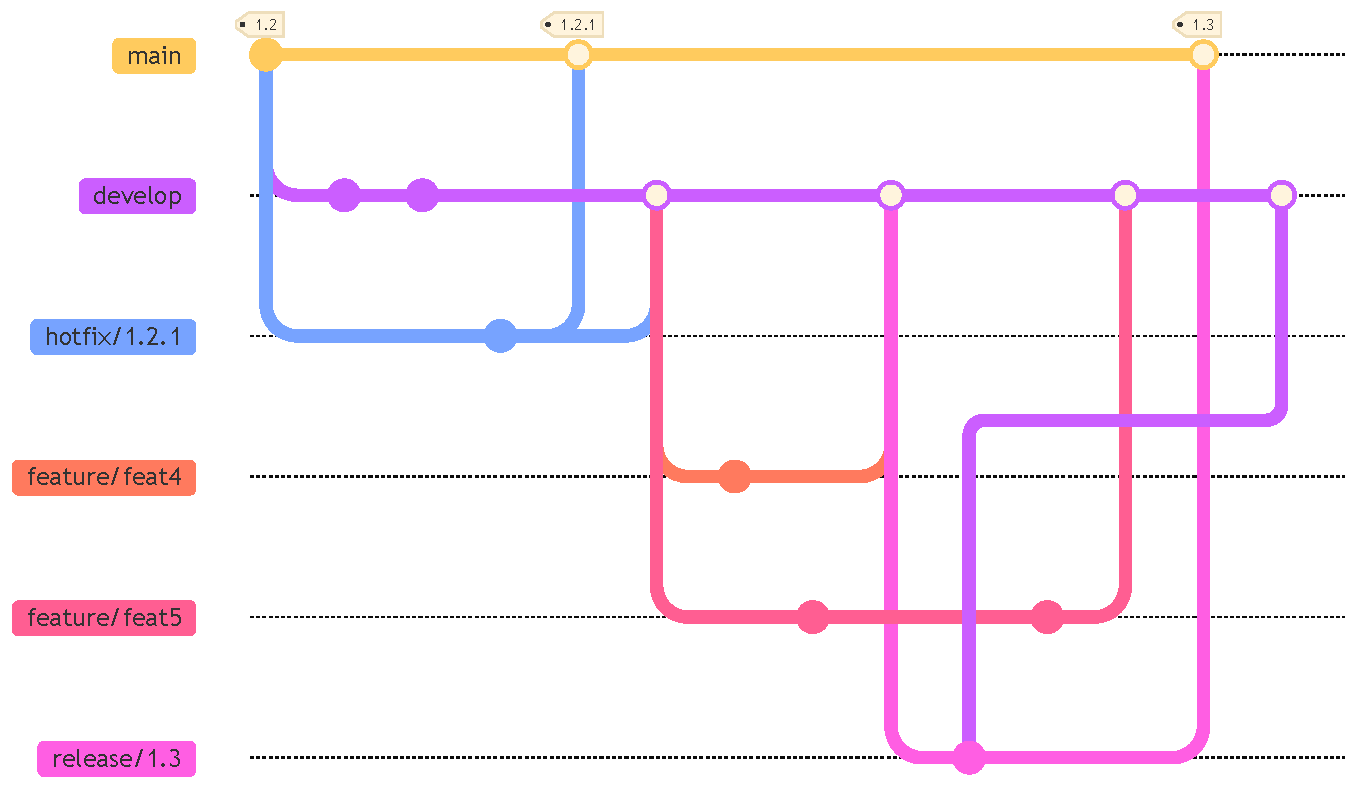
\includegraphics[width=0.7\linewidth]{src/assets/diagrams/gitflow/flow.pdf}
    \caption{Beispiel für Release- und Hotfix\hyp Branches in Gitflow}
    \label{fig:gitflow:flow}
    \Description{}
\end{figure*}

Ein beispielhafter Ablauf ist in \autoref{fig:gitflow:flow} dargestellt. Dabei werden zwei Features -- \texttt{feature/feat4} und \texttt{feature/feat5} -- parallel entwickelt. Feature 4 ist zuerst fertig und wird in \texttt{develop} integriert während sich Feature 5 noch in der Entwicklung befindet. Durch die Eröffnung von \texttt{release/1.3} wird ein neuer Release mit der Versionsnummer 1.3 gestartet. Da keine weiteren Features in den Release aufgenommen werden dürfen, muss Feature 5 auf den nächsten Release warten und darf nicht in den Release\hyp Branch aufgenommen werden.

Auf dem Release\hyp Branch wird ein Commit hinzugefügt, um bspw. die Versionsnummer zu erhöhen etc. Danach sind die Vorbereitungen für den Release abgeschlossen und der Branch wird in \texttt{main} integriert. Dieser Merge ist per Definition ein Release. Daher muss ein Tag für den Commit mit der neuen Versionsnummer erstellt werden. Außerdem wird der Release\hyp Branch auf \texttt{develop} integriert (\emph{Back\hyp Merge}), um die Änderungen zu reflektieren. Anschließend gilt der Release als abgeschlossen und der \texttt{release/1.3}-Branch wird gelöscht.

Durch die Einführung von Releases auf einen dedizierten Branch ist das \emph{Polishing} des Releases unter gleichzeitiger Weiterentwicklung auf \texttt{develop} ggf. durch unterschiedliche Teams möglich. Außerdem werden somit die Entwicklungs- bzw. Release\hyp Phasen wohl definiert und im Repository reflektiert~\cite{atlassianGitflowWorkflow}.


\subsubsection{Hotfix-Branches}

Die letzte Branch-Gruppe besteht in den Hotfixes. Diese verhalten sich ähnlich zu Feature- und Release\hyp Branches. Allerdings liegt der Ursprung von diesen in \texttt{main} und \emph{nicht} in \texttt{develop}. Ihre Notwendigkeit begründet sich in Szenarien, in denen es notwendig ist, schnell zu handeln basierend auf einem ungewollten Zustand in einer \emph{Live-Production-Version}, bspw. einem kritischen Fehler. Somit kann ein neuer ungeplanter Release vorbereitet werden (\emph{Hotfix-Release}). Entscheidend ist hierbei, dass die Arbeit auf \texttt{develop} nicht gestört wird, damit die Fehlerbehebung ggf. von einem anderen Team oder Entwickler:in durchgeführt werden kann.

Nach Erhöhung der Versionsnummer und Fertigstellung des Hotfixes wird der Branch in \texttt{main} integriert und mit einem entsprechenden Tag versehen. Außerdem muss ein Merge in \texttt{develop} stattfinden, außer es existiert bereits ein neuer \texttt{release}-Branch. In diesem Fall wird der Hotfix schließlich durch den \emph{Back-Merge} in \texttt{develop} integriert~\cite{driessenSuccessfulGitBranching2010}.

Ein Beispiel für einen Hotfix\hyp Branch\hyp Ablauf ist in \autoref{fig:gitflow:flow} dargestellt. Dabei wird von der Version \verb|1.2| von \texttt{main} der Branch \texttt{hotfix/1.2.1} abgezweigt. Der hypothetische Fehler wird behoben und ein Commit erstellt. Dieser wird direkt in \texttt{main} integriert und der zugehörige Tag mit der Versionsnummer erstellt. Außerdem wird er in \texttt{develop} integriert, um die Fehlerbehebung beizubehalten. Dabei beachte man die zwei Commits auf \texttt{develop}, welche in der Zwischenzeit hinzugefügt wurden. Diese sollen zwei weitere Features andeuten, welche parallel integriert worden sind. Es ist zu erkennen, dass die Entwicklungsarbeit an weiteren Features ungestört weiterlaufen kann.


\subsubsection{Fazit}

Insgesamt wurde Gitflow für versionierte Projekte entwickelt und nicht für kontinuierlich ausgelieferte Software~\cite{driessenSuccessfulGitBranching2010}, wie bspw. mobile Anwendungen. Daher wird dieses Vorgehensmodell für veraltet, aber von historischer Bedeutung gesehen~\cite{atlassianGitflowWorkflow}. Aufgrund der Schwierigkeiten mit \emph{Continuous Integration / Continuous Deployment} und da moderne Software meist kontinuierlich ausgeliefert wird, wird oft das Vorgehensmodell der Trunk-based Development (vgl. \autoref{sec:workflows:trunk}) bevorzugt~\cite{atlassianGitflowWorkflow}. Dennoch wird es für Projekte mit einem geplanten Release-Rhythmus immer noch für geeignet gehalten~\cite{atlassianGitflowWorkflow,driessenSuccessfulGitBranching2010}.

Da Features erst nach der Fertigstellung in \texttt{develop} mittels no\hyp fast\hyp forward\hyp Merge integriert werden, entstehen große Commits. Daher ist ein höheres Risiko an Merge\hyp Konflikten sowie an Abweichungen von \texttt{main} gegeben~\cite{atlassianGitflowWorkflow}. Dennoch wird damit die Übersichtlichkeit und eindeutige Identifikation von Commit zu Feature gewährleistet.

Gitflow und das Feature\hyp Branching\hyp Modell teilen sich die gemeinsame Basis eines Haupt\hyp Branches und verschiedener, dedizierter Feature\hyp Branches. Daher sind alle Vorteile, wie bspw. die Möglichkeit von isolierten Experimenten und die effiziente Kollaboration, hier ebenfalls gegeben.

Ein Vorteil liegt im Fokus auf Release\hyp vorbereitenden Tätigkeiten, welche getrennt vom restlichen Entwicklungsprozess stattfinden können. Außerdem stellen Hotfix\hyp Branches einen dedizierten Kanal für \emph{Patches} auf \emph{Production} dar~\cite{atlassianGitflowWorkflow}.
